\documentclass[10pt,a4paper]{article}

\usepackage[spanish]{babel}
\usepackage[utf8]{inputenc}
\usepackage{geometry}
\usepackage{url}
\usepackage{amsmath}
\usepackage{graphicx}
\usepackage{float}
\usepackage{listings}
\usepackage{color}
\usepackage{multicol}
\definecolor{grey}{rgb}{0.8,0.8,0.8}
\usepackage{listings}
\usepackage{color,soul}
\usepackage{caption}
\usepackage{subcaption}
\usepackage{pdfpages}
%\usepackage{DejaVuSans}
%\usepackage{DejaVuSansMono}
%\renewcommand*\familydefault{\ttdefault}

%\lstset{basicstyle=\footnotesize\ttfamily,breaklines=true}
%\lstset{framextopmargin=50pt,frame=bottomline}
\geometry{left=1.0in,right=1.0in,top=1.0in,bottom=1.0in }

\lstset{
  frame=top,frame=bottom,
  basicstyle=\footnotesize\normalfont\ttfamily,%\sffamily,    % the size of the fonts that are used for the code
  stepnumber=1,                           % the step between two line-numbers. If it is 1 each line will be numbered
  numbersep=10pt,                         % how far the line-numbers are from the code
  tabsize=2,                              % tab size in blank spaces
  extendedchars=true,                     %
  breaklines=true,                        % sets automatic line breaking
  captionpos=t,                           % sets the caption-position to top
  mathescape=true,
  stringstyle=\color{white}\ttfamily, % Farbe der String
  showspaces=false,           % Leerzeichen anzeigen ?
  showtabs=false,             % Tabs anzeigen ?
  xleftmargin=17pt,
  framexleftmargin=17pt,
  framexrightmargin=17pt,
  framexbottommargin=5pt,
  framextopmargin=5pt,
  showstringspaces=false      % Leerzeichen in Strings anzeigen ?
 }
 
% Macros
% #1 : Path of image. eg : window/aWindow.png
% #2 : Caption of image. eg : a caption
% #3 : Width of image in centimeters. eg : 15
% #4 : Height of image in centimeters. eg : 20
% 
% example : \presentgrafic{window/aWindow.png}{caption}{15}{20}
\newcommand{\presentgrafic}[4]{
\begin{figure}[H]
\centering
\includegraphics[width=#3cm, height=#4cm]{#1}
\caption{#2}
\label{fig:my_label}
\end{figure}
}

\begin{document}

% No nos olvidemos de imprimir la caratula del TP c:
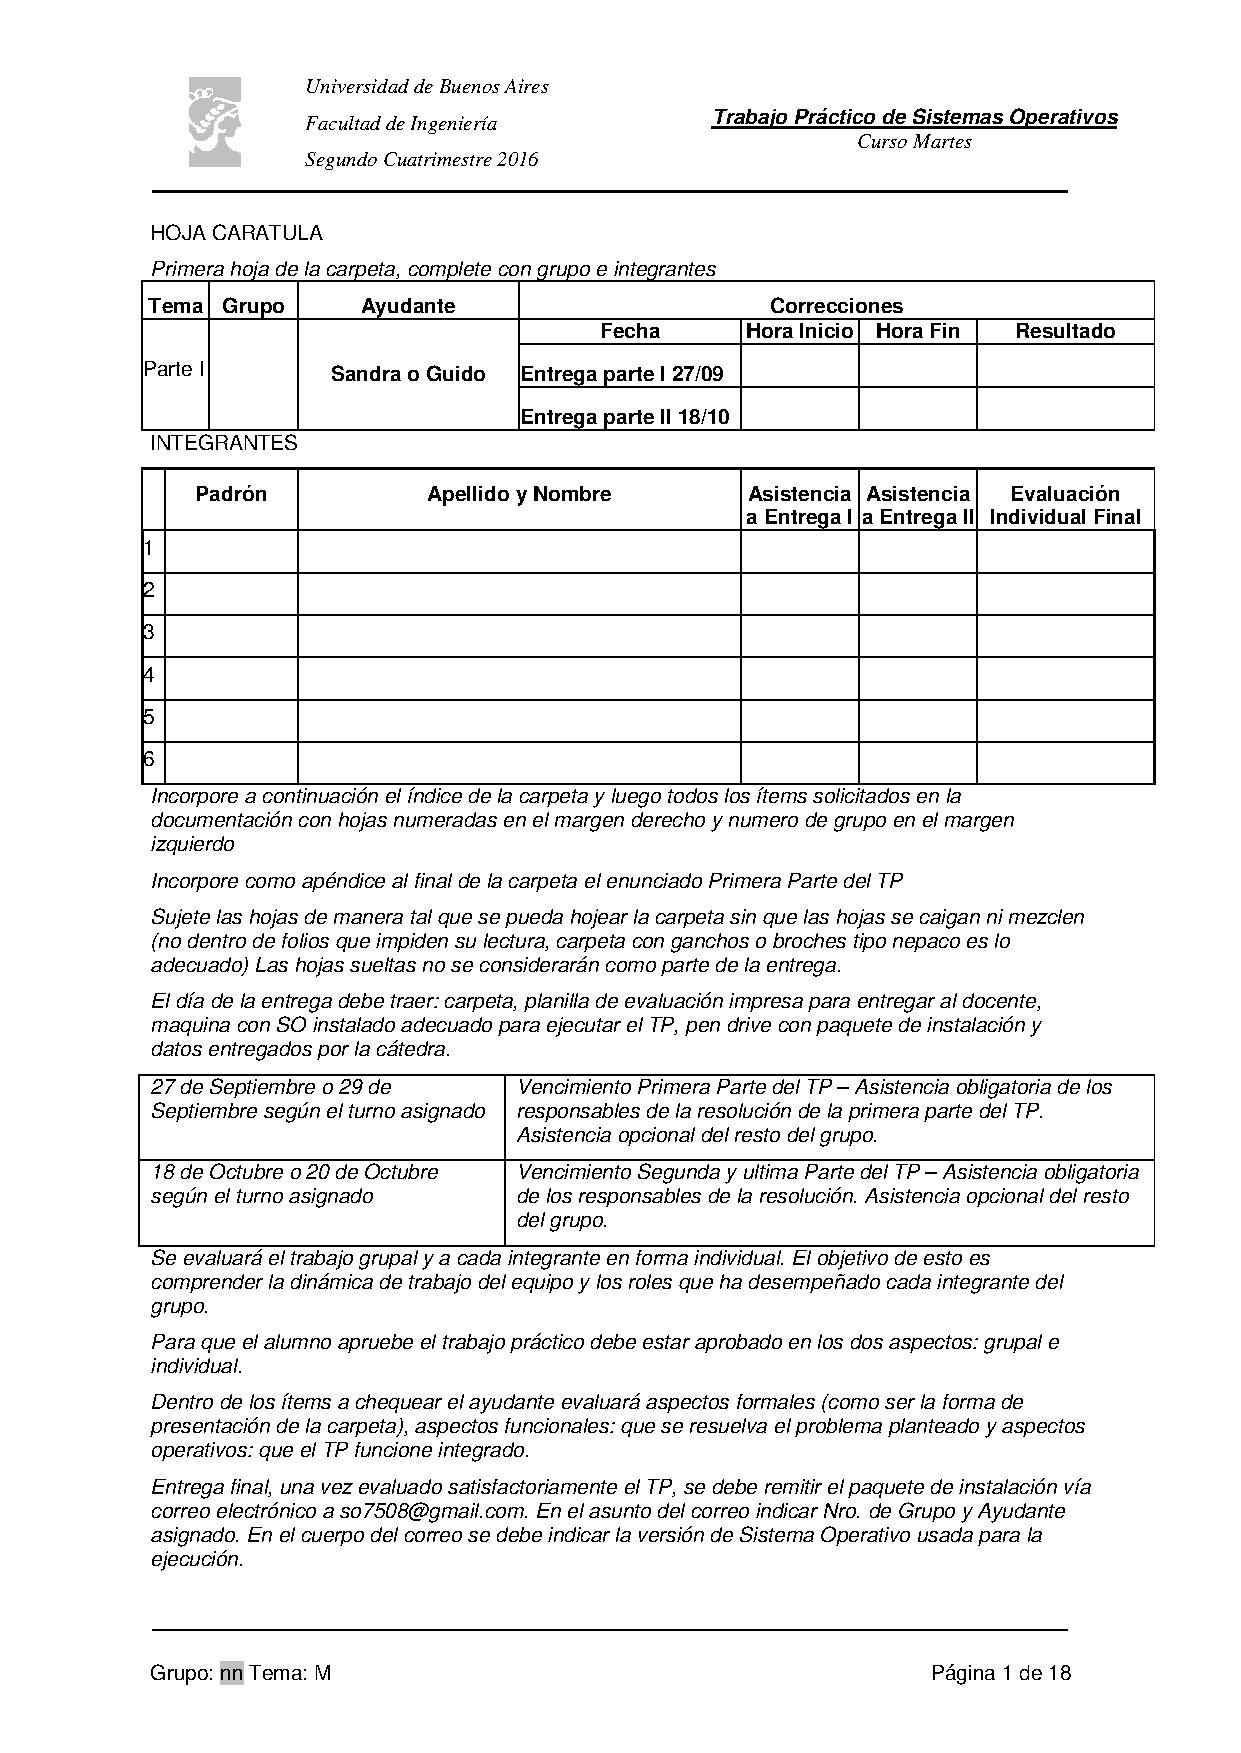
\includepdf[pages={1-1}]{enunciado/parte1.pdf}

\begin{titlepage}

\newcommand{\HRule}{\rule{\linewidth}{0.5mm}} % Defines a new command for the horizontal lines, change thickness here

\center % Center everything on the page

\textsc{\LARGE Facultad de Ingeniería - UBA}\\[1.5cm]
\textsc{\Large Sistemas Operativos 75.08}\\[0.5cm]
\textsc{\large Trabajo Práctico: Primera Entrega}\\[0.5cm]

\HRule \\[0.4cm]
{ \huge \bfseries EPLAM}\\[0.4cm]
\HRule \\[1.5cm]

\begin{minipage}{0.5\textwidth}
\begin{flushleft} \large
\emph{Integrantes:}\\
Agustina \textsc{Barbetta} \textit{96528}\\
Ana \textsc{Czarnitzki} \textit{96812}\\
Francisco \textsc{Ordoñez} \textit{96478}\\
Manuel \textsc{Porto} \textit{96587}\\
Santiago \textsc{Aguilera} \textit{95795}\\
\end{flushleft}
\end{minipage}
~
\begin{minipage}{0.4\textwidth}
\begin{flushright} \large
\emph{Mails:}\\
\texttt{agustina.barbetta@gmail.com}\\
\texttt{czarniana@gmail.com}\\
\texttt{ordonez.f93@gmail.com}\\
\texttt{manu.porto94@gmail.com}\\
\texttt{marquito.santi@gmail.com}\\
\end{flushright}
\end{minipage}\\[2cm]

{\Large \texttt{Grupo 6}}\\[2cm]

\selectlanguage{spanish}
{\large \today}\\[3cm]


%\includegraphics{Logo}\\[1cm]

\vfill % Fill the rest of the page with whitespace

\end{titlepage}

\pagebreak

\tableofcontents

\pagebreak

\section{Aclaraciones Globales e Hipótesis por comando}
% Documente cualquier aclaración que considere necesaria para asegurar el éxito de la corrección
% Documente las hipótesis que ha considerado para la resolución en cada comando (opcional)
% Si no hay aclaraciones ni hipótesis, igualmente incorpore esta hoja con solo su titulo aka \pagebreak
Para el correcto funcionamiento del aplicativo se deben cumplir los siguientes requisitos:

\begin{enumerate}
    \item Bash v4 o superior
    \item Perl v5.10.0 o superior
    \item Sistema Operativo Linux
\end{enumerate}

\section{Problemas relevantes}
% Describa los problemas relevantes que se hayan presentado durante el desarrollo, la integración y/o la prueba del sistema. Explique cómo fueron solucionados.
Como primer y principal problema podemos destacar la dificultad de escribir código bash común para los diferentes sistemas operativos. En nuestro caso programamos tanto en Mac OS como Linux y dado que no pudimos encontrar un método que funcione en todas las computadoras (en particular para el comando du -b, que pudimos utilizar en la segunda y no así en la primera distribución) decidimos utilizar la versión para Linux ya que este es el sistema operativo con el que generalmente estuvimos trabajando en materias anteriores.\\
En el caso de Windows, se pudo correr el \texttt{EPLAM} satisfactoriamente, pero solo para la distribución \texttt{Windows 10} y haciendo uso del \textit{Windows Subsystem for Linux}.\\ 
Otro problema que tuvimos, al momento de realizar la primera entrega de este trabajo, fue el hecho de que el mismo no tiene todos los comandos programados. De esta manera, hay ciertas funciones que nos hubieran sido más sencillas de probar si contáramos con una solución global. Específicamente, en el \texttt{Installep} nos hubiera servido tener hecho el \texttt{Movep}.\\
Al momento de realizar la segunda entrega subsanamos este primer problema al ya tener todo el sistema como un conjunto, facilitándo la integración entre las distintas partes.

\section{README}
% OBLIGATORIO que en la carpeta se incluya la impresión del README, el docente seguirá estos pasos para instalar y ejecutar el TP
\textbf{Adjunto por separado}

\section{Listado de Nuevas Funciones y/o Comandos Auxiliares}
% Si agrega funciones o comandos auxiliares, Indique: Nombre de la función, quienes la usan, para que la usan.

\subsection{Installep}
El comando \texttt{Installep.sh} utiliza varias funciones, cada una representa uno de los puntos del enunciado, de modo que las mismas son:

\begin{itemize}
    \item input\_directories.
    \item system\_already\_installed.
    \item set\_news\_size.
    \item show\_values.
    \item instalation\_confirm.
    \item installation.
    \item create\_conf\_archive.
    \item end\_process.
\end{itemize}

Cada una de ellas se encuentra documentada en el código fuente.\\
A eso se le suma un main, el \texttt{Installep} propiamente dicho, que ejecuta a cada una de las anteriores de forma secuencial, pidiendo las validaciones correspondientes (que devuelvan 0 o 1 para el caso de system\_already\_installed y aquellas que esperan confirmaciones por parte del usuario) y volviendo atrás en el caso de ser necesario.\\
Existen algunas funciones más pero que podrían considerarse auxiliares llamadas \texttt{input\_directory} y \texttt{directory\_already\_exists}. La primera espera del usuario un nombre para un directorio y sobre-escribe una variable pasado por parámetro en el caso de que la cadena escrita sea distinta de \texttt{config} dado que el mismo es un valor reservado. Por otro lado, la ultima mencionada verifica que el directorio propuesto por el usuario no exista previamente.

\subsection{Initep}
El comando \texttt{Initep.sh} se implementa con una función auxiliar por paso requerido en el enunciado del trabajo. Cada función realiza una única tarea, devolviendo 0 en caso de éxito o 1 en caso contrario. Al final del \textit{script}, se invoca a cada función y se evalúa su retorno. En caso de falla, se destruye el ambiente creado (\texttt{unset} de cada variable exportada) y se retorna un código de salida específico.\\
Para verificar una inicialización previa de las variables de entorno, se crea una variable adicional \texttt{ENV}, a la cual se le asigna el valor 1 al momento de la inicialización. De esta forma, en cada ejecución del comando, se verifica si \texttt{ENV} es equivalente a 1. En este caso, se detiene \texttt{Initep} notificando al usuario que las variables ya fueron inicializadas y exportadas.\\
Las funciones auxiliares se encuentran documentadas en el código fuente.

\subsection{Demonep}
El daemon es el encargado de estar corriendo siempre en segundo plano (para ello se lo necesita ejecutar agregando al final un \texttt{\&}). Sus tareas consisten en:

\begin{itemize}
    \item  Verificar si hay nuevos archivos dentro del directorio de novedades \texttt{\$DIRREC}
    
    \item Validar cada archivo si es apto para ser procesado, moviendolo de directorios de acuerdo al estado de su validacion
    
    \item Invocar a la función \texttt{Procep.sh} si hay archivos validos a ser procesados.
\end{itemize}

El \textit{script} corre en ciclos con un tiempo de espera de 15 segundos. Esto quiere decir que el mismo cada 15 segundos realizara ``pasadas'' a la carpeta de novedades y validara los archivos internos.

La forma de validación es la siguiente:

\begin{enumerate}
    \item Ver que el archivo comience con \texttt{ejecutado\_} y tenga la extensión correcta \texttt{.csv}.
    
    \item Ver que el archivo tenga el año presupuestario corriente. En este caso será 2016. El mismo se adapta al año corriente (no es un numero mágico)
    
    \item Ver que el archivo tenga un código de provincia valido. Los códigos se reciben del archivo \texttt{\$DIRMAE}/provincias.csv. Si el código de la provincia no se encuentra dentro del csv, no sera correcto
    
    \item Ver que la fecha sea mayor a la del año presupuestario pero menor a la actual. Para ello se validara de la siguiente forma:
    
    \begin{itemize}
        \item El año debe ser el corriente
        
        \item Si es el mismo mes, el día no debe ser mayor al actual
        
        \item Si es otro mes, el mes no debe ser mayor al actual
        
        \item Validar que la fecha este bien formada y con el formato pedido (YYYYmmdd)
    \end{itemize}
    
\end{enumerate}

Las validaciones se hacen en el orden descrito. Si alguna de ellas falla, la única que se reportará en el \textit{log} será la primera ocurrencia. 

Un ejemplo de archivo correcto seria:

\texttt{ejecutuado\_2016\_4\_20160809.csv}

Si el archivo es correcto, el mismo se moverá al directorio \texttt{\$DIROK}, caso contrario se encontrara en \texttt{\$DIRNOK}. Para ello se hará uso del \textit{script} \texttt{Movep.sh}.

Finalmente, siempre y cuando haya archivos dentro de \texttt{\$DIROK}, si el script \texttt{Procep.sh} no se encuentra en ejecucion, se ejecutara el mismo para que procese los archivos validos. Si ya se encuentra en ejecucion, se postergara para el proximo ciclo del daemon.

Cabe notar que el daemon guardará en un \textit{log} todos los movimientos de archivos que realice y acciones (incluyendo información especifica de que fue lo que fallo en caso de haber errores). Para eso hará uso del \textit{script} \texttt{Logep.sh}

\subsection{Logep}
El comando \texttt{Logep} escribe la informacion indicada en distintos archivos de log, dependiendo del comando que este logeando la informacion. El ejecutable provee sus instrucciones de uso:

\begin{lstlisting}
Uso: Logep.sh -c comando -m 'Mensaje' -t tipo de mensaje
Ejemplo: Logep.sh -c movep -m 'Se movio archivo foo' -t INF 
  -h                  Muestra este mensaje de ayuda.
  -c comando          Escribir el mensaje en comando.log.
  -m 'Mensaje'        Mensaje a escribir.
  -t tipo de mensaje  Especifica el tipo de mensaje. Puede ser INF (tipo default), WAR, ERR. (Parametro opcional)
\end{lstlisting}

Si bien para la implementación del comando, \texttt{Logep.sh} no se programaron comandos auxiliares, si se utilizaron comandos provistos por el sistema operativo. Estos son:

\begin{enumerate}
    \item \texttt{du} para obtener el espacio disponible en disco.
    \item \texttt{tail} para obtener las ultimas \textit{n} lineas y conservarlas en el archivo de log cuando el mismo es reducido.
    \item \texttt{getopts} para poder parsear los argumentos por linea de comandos.
\end{enumerate}


Además de esto se implementaron funciones con el objetivo de encapsular código repetido y simplificar el código fuente del comando.

\begin{enumerate}
    \item \texttt{show\_help}
    \item \texttt{max\_log\_size\_reached}
    \item \texttt{reduce\_log\_file}
    \item \texttt{write\_log\_file}
\end{enumerate}

\subsection{Movep}

Movep es el encargado de mover archivos de un directorio a otro. El mismo puede recibir por parametros a la hora de ser invocado los siguientes argumentos

\begin{itemize}
    \item c: Comando que lo invoco
    
    \item o: Origen
    
    \item d: Destino
\end{itemize}

\texttt{Movep} se encargara de mover el archivo del origen al destino, y loggear el resultado de la operación. Si se provee de un comando a la hora de invocarlo, el mismo loggeara bajo el nombre de ese comando. Caso contrario se creara bajo el \textit{log} de \texttt{Movep}.

El script valida ciertos casos de uso que no pueden darse. Los mismos son:

\begin{enumerate}
    \item Origen no existente (o vacío)
    
    \item Destino no existente (o vacío)
    
    \item Origen y destino iguales
\end{enumerate}

Si ocurre alguno de los mismos, el proceso se detendrá y se creara una entrada en el \textit{log} del error ocurrido.

A su vez, si el archivo ya se encuentra en el directorio destino, el mismo se creara bajo un subdirectorio \texttt{dpl}, usando un sufijo de incremento para poder diferenciarlos. Un ejemplo sería:


\begin{lstlisting}
# El archivo.csv se mueve correctamente a carpeta/
> bash Movep.sh -o archivo.csv -d carpeta/
# El archivo.csv ya existe en carpeta/, se crea dpl/ y se guarda archivo.csv alli
> bash Movep.sh -o archivo.csv -d carpeta/
# El archivo.csv ya existe en carpeta/ y en dpl/, se guarda dentro de 
dpl archivo.1.csv
> bash Movep.sh -o archivo.csv -d carpeta/
# El archivo.csv se mueve correctamente a carpeta/
> bash Movep.sh -o archivo.csv -d carpeta/
# El archivo.csv ya existe en carpeta/, se crea dpl/ y se guarda archivo.csv alli
> bash Movep.sh -o archivo.csv -d carpeta/
# El archivo.csv ya existe en carpeta/ y en dpl/, se guarda dentro de dpl archivo.1.csv
> bash Movep.sh -o archivo.csv -d carpeta/
\end{lstlisting}

\subsection{Procep}
El propósito de este proceso es reunir en un solo archivo todos los registros de presupuesto ejecutado validos 
\begin{itemize}
    \item Es el tercero en orden de ejecución y es invocado por Demonep.
    \item Graba los registros validos en un archivo de salida.
    \item Graba los registros rechazados en un archivo de rechazos indicando su motivo.
\end{itemize}
Luego de verificar que los archivos procesados por \texttt{Demonep} tengan la estructura correcta, \texttt{Procep} carga los archivos maestros en distintas tablas de hash para su fácil acceso en el momento de la verificación, luego procesa cada registro de cada archivo verificando que sus campos sean correctos.

Cada campo tiene una función que lo verifica, si el valor del campo \texttt{no} se encuentra en su tabla de hash se concatena el error a una variable que se usa en todas las verificaciones. Al finalizar el checkeo, si esa variable está vacia, el registro es correcto y se lo graba en el archivo de aceptados, caso contrario, al archivo de rechazados.

Al finalizar todos los registros de un archivo, se escribe en el log cuántos se validaron, cuántos son correctos y cuántos erróneos.

Las descripciones de los errores se encuentran en una tabla de hash.

\subsection{Listep}
El propósito de este proceso es generar diferentes listados de control entre el presupuesto 
sancionado y el presupuesto ejecutado. Tambien permite generar listados de control en base a distintos archivos de cotizaciones y años presupuestarios.
\begin{itemize}
    \item Es el cuarto en orden de ejecución y se dispara manualmente.
    \item Es el unico proceso que no graba en el archivo de log.   
\end{itemize} 

El mismo dependiendo de la opción seleccionada permite aplicarle filtros para el orden en el que las entries serán mostradas, o filtrar por distintos campos a procesar (dependiendo la opción seleccionada se puede filtrar por trimestres o por centros, entre otros).

El mismo permite una opción para poder guardar la salida en algún archivo. El formato a ser guardado sera en csv, con ";" de separador. Siempre va a estar también entregando la salida por \texttt{stdout}.

\section{Listado de Nuevos Archivos}
% Si agrega archivos NO TEMPORALES, Indique: Nombre del archivo, donde lo almacenan, quienes lo usan, para que lo usan.
El programa \texttt{Listep} crea diferentes archivos no temporales dependiendo de los flags con los que se lo ejecute.

\begin{enumerate}
    \item \texttt{perl Listep.pl --sanc [sanc\_file]} Crea un archivo \texttt{sancionado-yyyy.csv}.
    \item \texttt{perl Listep.pl --ejec [ejec\_file]} Crea un archivo sobre el presupuesto ejecutado (\texttt{ejecutado-yyyy.csv}).
    \item \texttt{perl Listep.pl --ctrl [ejec\_file] [sanc\_file]} Crea un reporte sobre el presupuesto en su conjunto.
\end{enumerate}
 
 En todos los casos los archivos son creados en el path donde fue ejecutado \texttt{Listep} y no son utlizados por otros comandos.
 
 Por su parte, el comando \texttt{Procep} crea dos archivos distintos, \texttt{ejecutado-yyyy.csv} donde se almacenan todos los registros validos y \texttt{rechazado-yyyy.csv} que contiene registros rechazados. El primer archivo es utilizado por \texttt{Listep}, mientras que el segundo no es utilizado por ningún comando. Ambos archivos son guardados en \texttt{\$DIRPROC}.

\section{Listado de DATOS}
% Imprima un listado con todos los nombres de los archivos de datos entregados por la cátedra y su cantidad de registros
Los archivos de datos utilizados por el aplicativo son los siguientes:

\textbf{Archivos maestros:}
\begin{description}
    \item [actividades.csv] con campos COD\_ACT, OBJ\_ACT, PGM\_ACT, NOM\_ACT y 33 entradas.
    \item [centros.csv] con campos COD\_CEN, NOM\_CEN y 17 entradas.

    \item [provincias.csv] con campos COD\_PROV, NOM\_PROV, REG\_PROV y 24 entradas.
    \item [sancionado-2016.csv] con campos COD\_CEN\_SAN, NOM\_TRI\_SAN, F11\_FIN\_SAN, F21\_FIN\_SAN y 68 entradas.
    \item [sancionado-2015.csv] con campos COD\_CEN\_SAN, NOM\_TRI\_SAN, F11\_FIN\_SAN, F21\_FIN\_SAN y 68 entradas.
    \item [tabla-AxC.csv] con campos ACT\_AXC, CEN\_AXC y 157 entradas.
    \item [trimestres.csv] con campos ANO\_TRI, NOM\_TRI, FDESDE\_TRI, FHASTA\_TRI y 10 entradas.
\end{description}

\textbf{Archivos novedades:}
\begin{description}
    \item [ejecutado\_2016\_*.csv] con campos ID\_EJE, FECHA\_EJE, COD\_CEN\_EJE, NOM\_ACT\_EJE, NOM\_TRI\_EJE, GASTO\_EJE y distintas cantidades de entradas.
\end{description}

\section{Apéndice}
\subsection{Enunciado: Primera parte}
\includepdf[pages={2-}]{enunciado/parte1.pdf}

\subsection{Enunciado: Segunda parte}
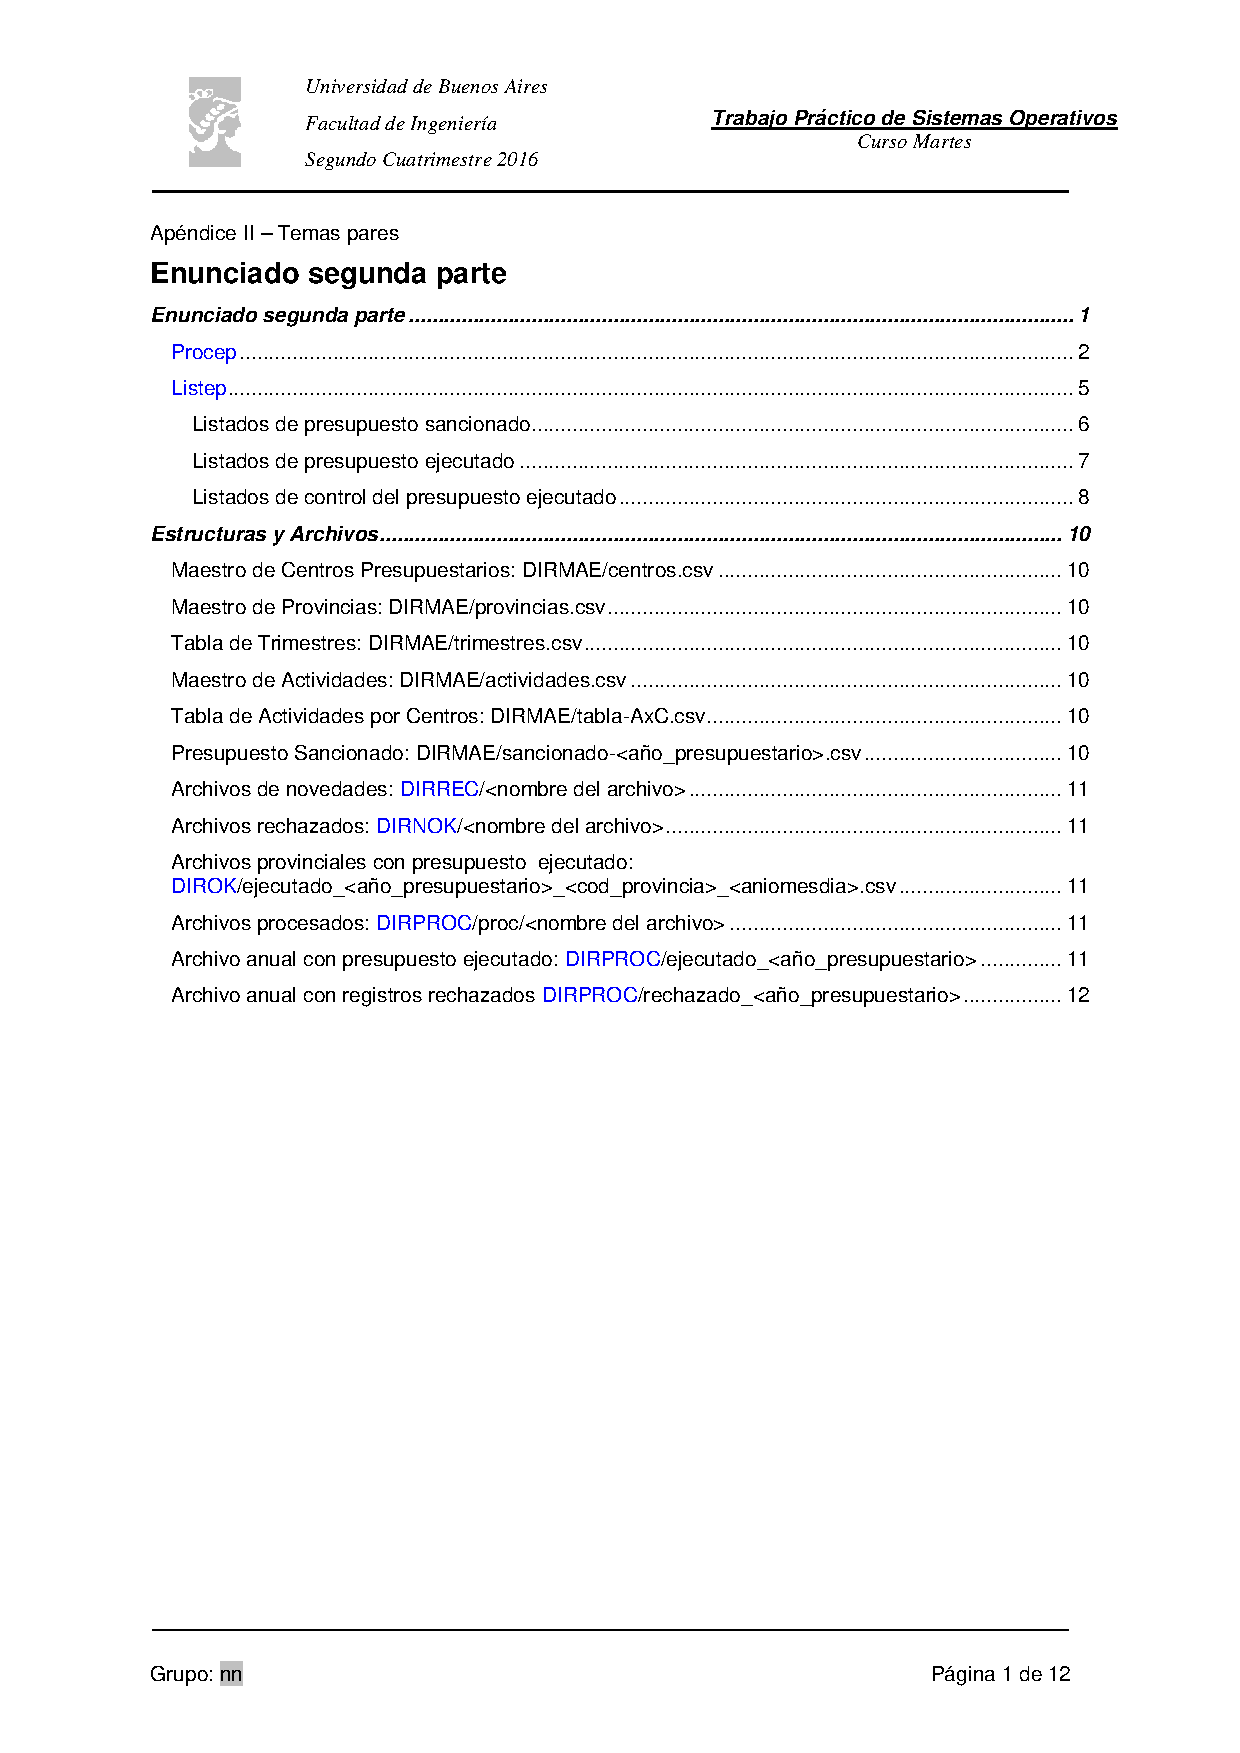
\includepdf[pages={-}]{enunciado/parte2.pdf}

\end{document}
